\documentclass[11pt,a4paper]{report}
\usepackage[textwidth=37em,vmargin=30mm]{geometry}
\usepackage{calc,xunicode,amsmath,amssymb,paralist,enumitem,tabu,booktabs,datetime2,xeCJK,xeCJKfntef,listings}
\usepackage{tocloft,fancyhdr,tcolorbox,xcolor,graphicx,eso-pic,xltxtra,xelatexemoji}

\newcommand{\envyear}[0]{2025}
\newcommand{\envdatestr}[0]{2025-02-25}
\newcommand{\envfinaldir}[0]{webdb/2025/20250225/final}

\usepackage[hidelinks]{hyperref}
\hypersetup{
    colorlinks=false,
    pdfpagemode=FullScreen,
    pdftitle={Web Digest - \envdatestr}
}

\setlength{\cftbeforechapskip}{10pt}
\renewcommand{\cftchapfont}{\rmfamily\bfseries\large\raggedright}
\setlength{\cftbeforesecskip}{2pt}
\renewcommand{\cftsecfont}{\sffamily\small\raggedright}

\setdefaultleftmargin{2em}{2em}{1em}{1em}{1em}{1em}

\usepackage{xeCJK,xeCJKfntef}
\xeCJKsetup{PunctStyle=plain,RubberPunctSkip=false,CJKglue=\strut\hskip 0pt plus 0.1em minus 0.05em,CJKecglue=\strut\hskip 0.22em plus 0.2em}
\XeTeXlinebreaklocale "zh"
\XeTeXlinebreakskip = 0pt


\setmainfont{Brygada 1918}
\setromanfont{Brygada 1918}
\setsansfont{IBM Plex Sans}
\setmonofont{JetBrains Mono NL}
\setCJKmainfont{Noto Serif CJK SC}
\setCJKromanfont{Noto Serif CJK SC}
\setCJKsansfont{Noto Sans CJK SC}
\setCJKmonofont{Noto Sans CJK SC}

\setlength{\parindent}{0pt}
\setlength{\parskip}{8pt}
\linespread{1.15}

\lstset{
	basicstyle=\ttfamily\footnotesize,
	numbersep=5pt,
	backgroundcolor=\color{black!5},
	showspaces=false,
	showstringspaces=false,
	showtabs=false,
	tabsize=2,
	captionpos=b,
	breaklines=true,
	breakatwhitespace=true,
	breakautoindent=true,
	linewidth=\textwidth
}






\newcommand{\coverpic}[2]{
    % argv: itemurl, authorname
    Cover photo by #2~~(\href{#1}{#1})
}
\newcommand{\makeheader}[0]{
    \begin{titlepage}
        % \newgeometry{hmargin=15mm,tmargin=21mm,bmargin=12mm}
        \begin{center}
            
            \rmfamily\scshape
            \fontspec{BaskervilleF}
            \fontspec{Old Standard}
            \fontsize{59pt}{70pt}\selectfont
            WEB\hfill DIGEST
            
            \vfill
            % \vskip 30pt
            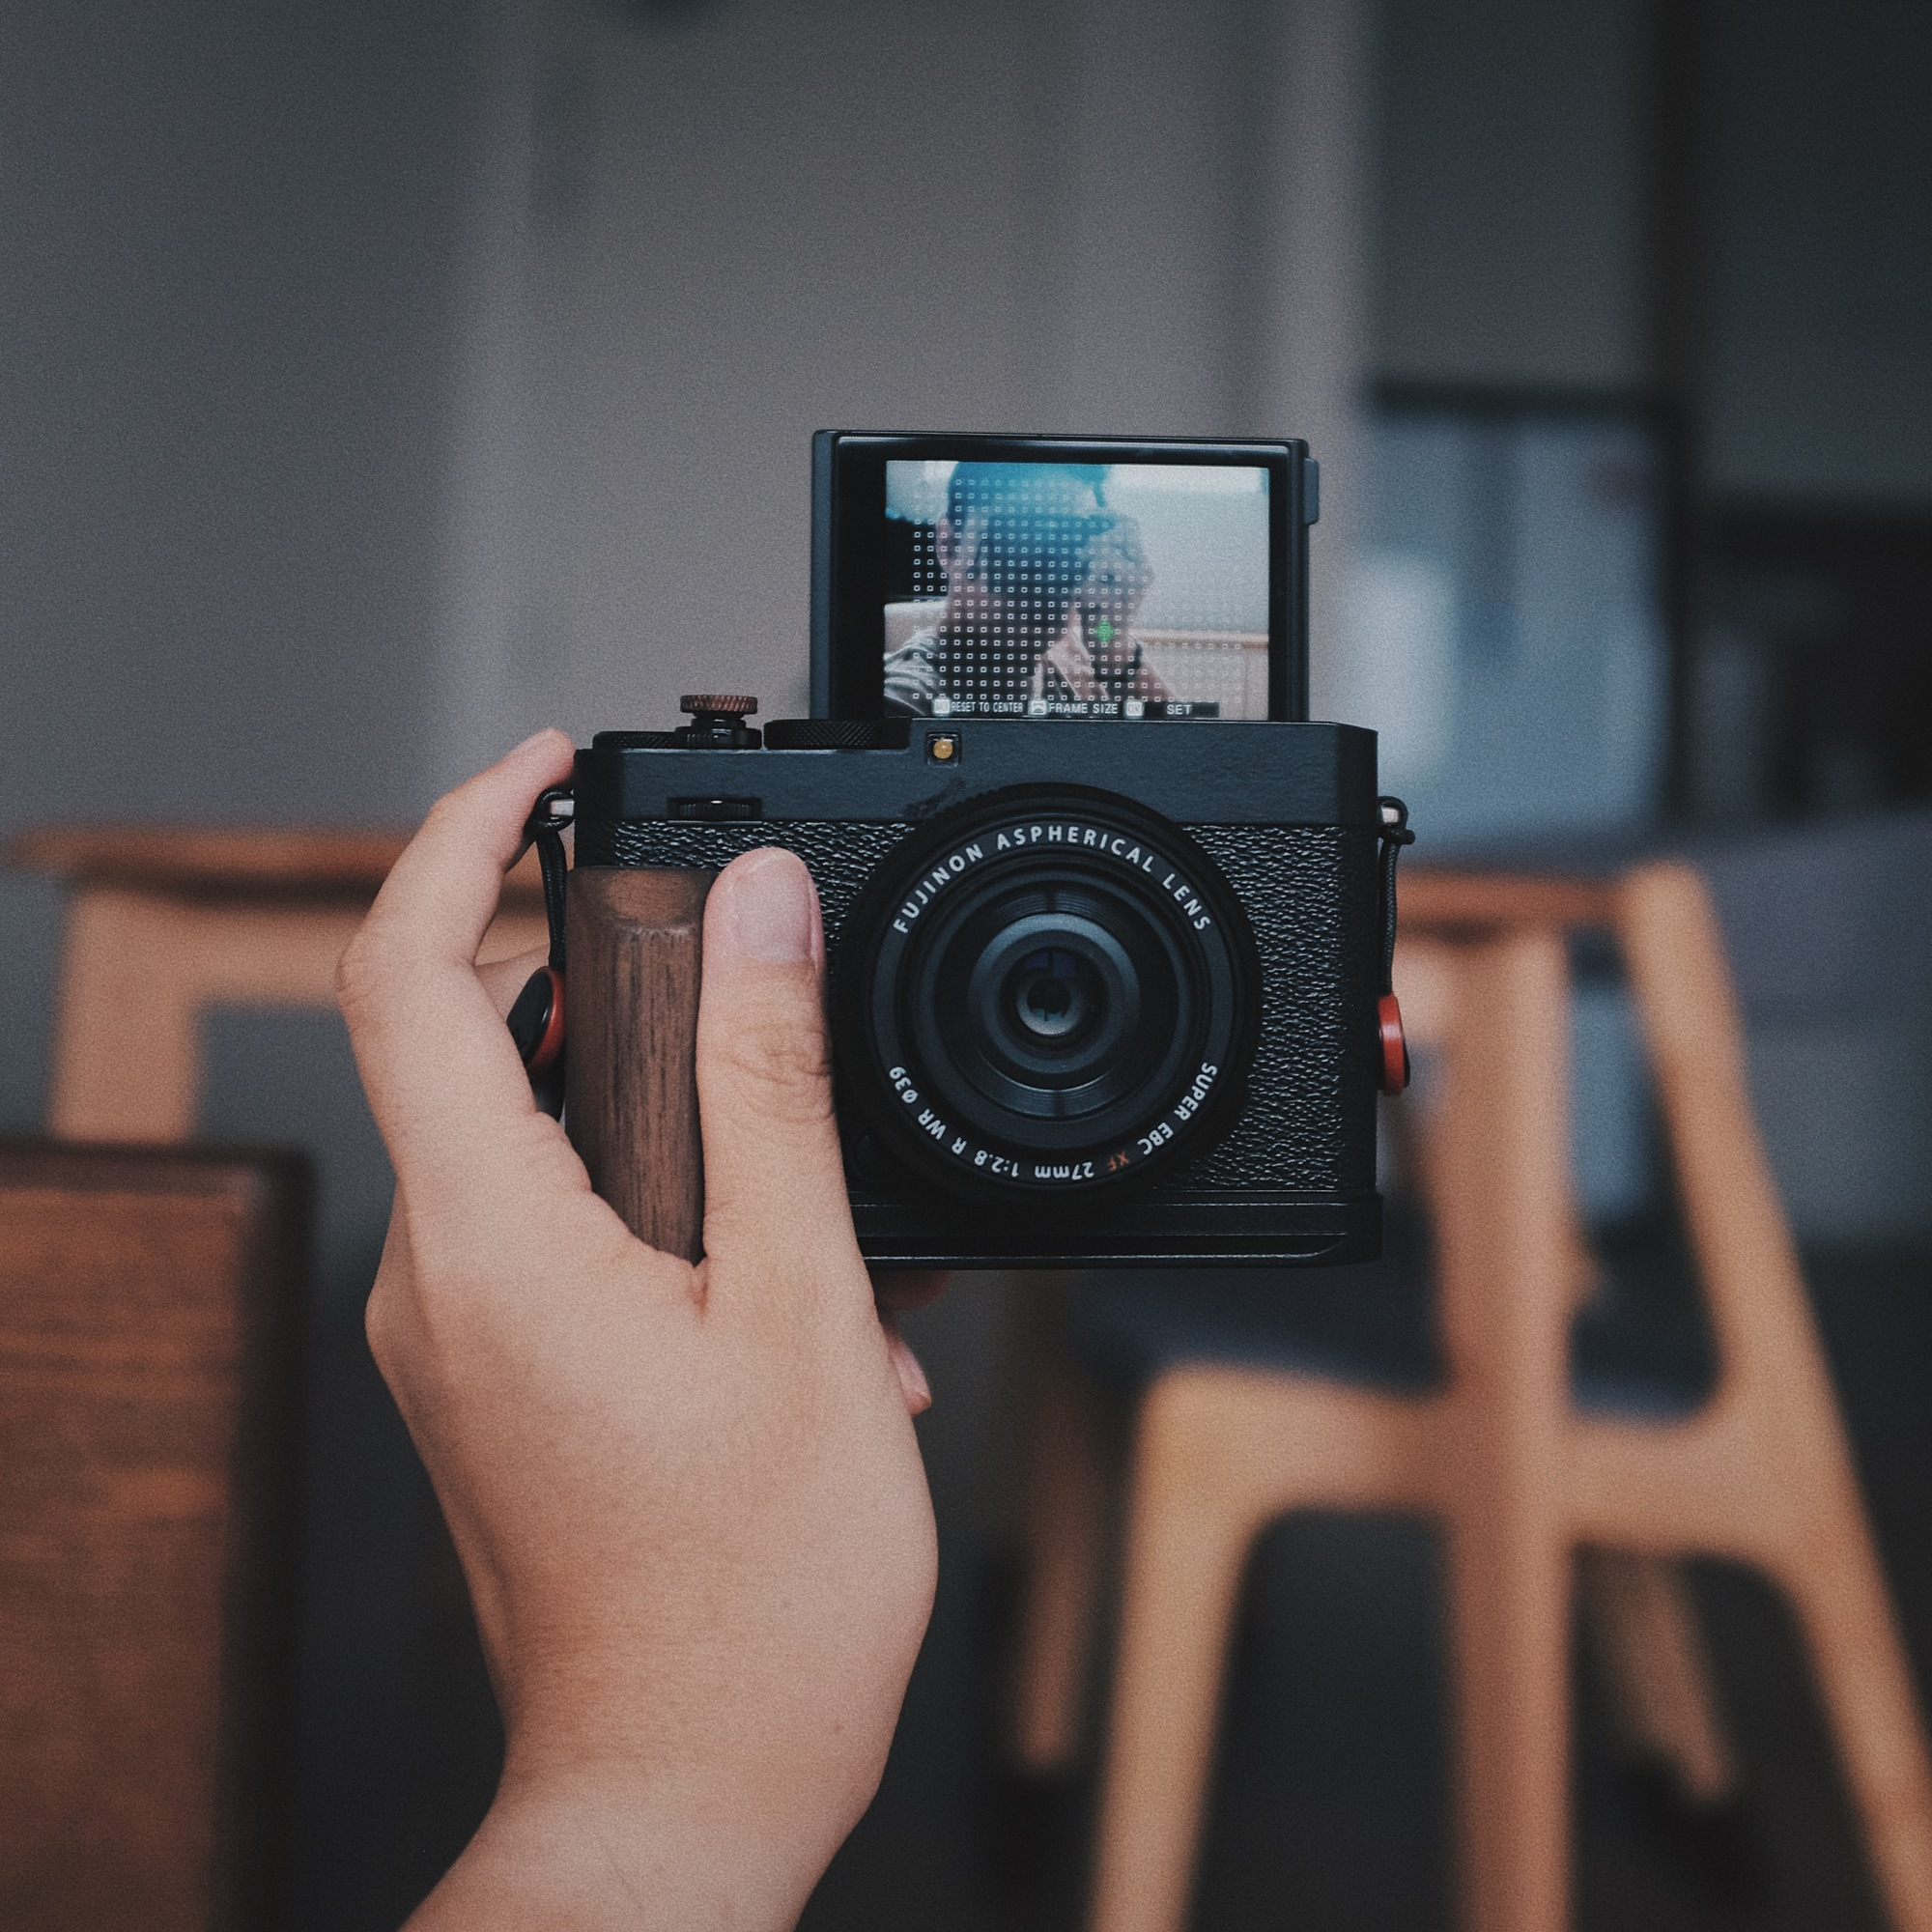
\includegraphics[width=\linewidth]{\envfinaldir/coverpic-prod.jpg}\par
            % \vskip 30pt
            \vfill

            \normalsize\rmfamily\scshape
            \copyright{} The Web Digest Project \hfill\large \envdatestr
        \end{center}
    \end{titlepage}
    % \restoregeometry
}
\newcommand{\simplehref}[1]{%
    \textcolor{blue!80!green}{\href{#1}{#1}}%
}
\renewcommand{\contentsname}{\center\Huge\sffamily\bfseries Contents\par\vskip 20pt}
\newcounter{ipartcounter}
\setcounter{ipartcounter}{0}
\newcommand{\ipart}[1]{
    % \vskip 20pt
    \clearpage
    \stepcounter{ipartcounter}
    \phantomsection
    \addcontentsline{toc}{chapter}{#1}
    % \begin{center}
    %     \Huge
    %     \sffamily\bfseries
    %     #1
    % \end{center}
    % \vskip 20pt plus 7pt
}
\newcounter{ichaptercounter}
\setcounter{ichaptercounter}{0}
\newcommand{\ichapter}[1]{
    % \vskip 20pt
    \clearpage
    \stepcounter{ichaptercounter}
    \phantomsection
    \addcontentsline{toc}{section}{\numberline{\arabic{ichaptercounter}}#1}
    \begin{center}
        \Huge
        \sffamily\bfseries
        #1
    \end{center}
    \vskip 20pt plus 7pt
}
\newcommand{\entrytitlefont}[1]{\subsection*{\raggedright\Large\sffamily\bfseries#1}}
\newcommand{\entryitemGeneric}[2]{
    % argv: title, url
    \parbox{\linewidth}{
        \entrytitlefont{#1}\par\vskip 5pt
        \footnotesize\ttfamily\mdseries
        \simplehref{#2}
    }\vskip 11pt plus 11pt minus 1pt
}
\newcommand{\entryitemGithub}[3]{
    % argv: title, url, desc
    \parbox{\linewidth}{
        \entrytitlefont{#1}\par\vskip 5pt
        \footnotesize\ttfamily\mdseries
        \simplehref{#2}\par\vskip 5pt
        \small\rmfamily\mdseries#3
    }\vskip 11pt plus 11pt minus 1pt
}
\newcommand{\entryitemAp}[3]{
    % argv: title, url, desc
    \parbox{\linewidth}{
        \entrytitlefont{#1}\par\vskip 5pt
        \footnotesize\ttfamily\mdseries
        \simplehref{#2}\par\vskip 5pt
        \small\rmfamily\mdseries#3
    }\vskip 11pt plus 11pt minus 1pt
}
\newcommand{\entryitemHackernews}[3]{
    % argv: title, hnurl, rawurl
    % \parbox{\linewidth}{
    %     \entrytitlefont{#1}\par\vskip 5pt
    %     \footnotesize\ttfamily\mdseries
    %     \simplehref{#3}\par
    %     \textcolor{black!50}{\href{#2}{#2}}
    % }\vskip 11pt plus 11pt minus 1pt
    \begin{minipage}{\linewidth}
            \entrytitlefont{#1}\par\vskip 5pt
            \footnotesize\ttfamily\mdseries
            \simplehref{#3}\par
            \textcolor{black!50}{\href{#2}{#2}}
    \end{minipage}\par\vskip 11pt plus 11pt minus 1pt
}







\begin{document}

\makeheader

\tableofcontents\clearpage




\ipart{Developers}
\ichapter{Hacker News}
\entryitemTwoLinks{"The closer to the train station, the worse the kebab" – a "study"}{https://news.ycombinator.com/item?id=43165112}{https://www.jmspae.se/write-ups/kebabs-train-stations/}

\entryitemTwoLinks{Claude 3.7 Sonnet and Claude Code}{https://news.ycombinator.com/item?id=43163011}{https://www.anthropic.com/news/claude-3-7-sonnet}

\entryitemTwoLinks{The best way to use text embeddings portably is with Parquet and Polars}{https://news.ycombinator.com/item?id=43162995}{https://minimaxir.com/2025/02/embeddings-parquet/}

\entryitemTwoLinks{Google Co-Scientist AI fed previous paper with the answer in it}{https://news.ycombinator.com/item?id=43162582}{https://pivot-to-ai.com/2025/02/22/google-co-scientist-ai-cracks-superbug-problem-in-two-days-because-it-had-been-fed-the-teams-previous-paper-with-the-answer-in-it/}

\entryitemTwoLinks{Show HN: I made a site to tell the time in corporate}{https://news.ycombinator.com/item?id=43162340}{https://corporate.watch}

\entryitemTwoLinks{Right to Repair laws have now been introduced in all 50 us states}{https://news.ycombinator.com/item?id=43161777}{https://www.ifixit.com/News/108371/right-to-repair-laws-have-now-been-introduced-in-all-50-us-states}

\entryitemTwoLinks{Larry Ellison's half-billion-dollar quest to change farming}{https://news.ycombinator.com/item?id=43161188}{https://www.wsj.com/tech/larry-ellison-hawaii-greenhouse-farm-food-2d260e1f}

\entryitemTwoLinks{Breaking into apartment buildings in five minutes on my phone}{https://news.ycombinator.com/item?id=43160884}{https://www.ericdaigle.ca/posts/breaking-into-dozens-of-apartments-in-five-minutes/}

\entryitemTwoLinks{Introduction to Stochastic Calculus}{https://news.ycombinator.com/item?id=43160779}{https://jiha-kim.github.io/posts/introduction-to-stochastic-calculus/}

\entryitemTwoLinks{Laravel Cloud}{https://news.ycombinator.com/item?id=43160612}{https://app.laravel.cloud/}

\entryitemTwoLinks{ARPA is funding cheap community-owned gigabit fiber to neglected neighborhoods}{https://news.ycombinator.com/item?id=43160196}{https://www.techdirt.com/2025/02/24/arpa-is-quietly-funding-cheap-50-65-a-month-community-owned-gigabit-fiber-access-to-long-neglected-neighborhoods/}

\entryitemTwoLinks{'Impossible-to-hack' security turns out to be no security}{https://news.ycombinator.com/item?id=43159544}{https://jltee.substack.com/p/new-zealand-companys-impossible-to-hack-security}

\entryitemTwoLinks{Show HN: I built an app to stop me doomscrolling by touching grass}{https://news.ycombinator.com/item?id=43158660}{https://touchgrass.now/}

\entryitemTwoLinks{Show HN: I scrape Steam data every month and it's yours to download for free}{https://news.ycombinator.com/item?id=43158425}{https://www.gginsights.io}

\entryitemTwoLinks{Is Ketamine Neurotoxic?}{https://news.ycombinator.com/item?id=43158292}{https://desmolysium.com/ketamineneurotoxic/}

\entryitemTwoLinks{Apple says it will add 20k jobs, spend \$500B, produce AI servers in US}{https://news.ycombinator.com/item?id=43158168}{https://www.bloomberg.com/news/articles/2025-02-24/apple-says-it-will-add-20-000-jobs-spend-500-billion-produce-ai-servers-in-us}

\entryitemTwoLinks{What's New in Emacs 30.1?}{https://news.ycombinator.com/item?id=43158164}{https://www.masteringemacs.org/article/whats-new-in-emacs-301}

\entryitemTwoLinks{Building a BitTorrent client from the ground up in Go (2020)}{https://news.ycombinator.com/item?id=43157980}{https://blog.jse.li/posts/torrent/}

\entryitemTwoLinks{Microsoft cancels leases for AI data centers, analyst says}{https://news.ycombinator.com/item?id=43157831}{https://www.bloomberg.com/news/articles/2025-02-24/microsoft-cancels-leases-for-ai-data-centers-analyst-says}

\entryitemTwoLinks{Cloudflare takes legal action over LaLiga's "disproportionate blocking efforts"}{https://news.ycombinator.com/item?id=43157000}{https://www.broadbandtvnews.com/2025/02/19/cloudflare-takes-legal-action-over-laligas-disproportionate-blocking-efforts/}\ichapter{Phoronix}
\entryitemGeneric{\hskip 0pt{}Armbian 25.2 Released With New Boards Supported, Kernel Upgrades}{https://www.phoronix.com/news/Armbian-25.2-Released}

\entryitemGeneric{\hskip 0pt{}Canonical Rolling Out Improved CLA Process For Ubuntu Contributions}{https://www.phoronix.com/news/Canonical-Better-CLA-Process}

\entryitemGeneric{\hskip 0pt{}Intel Linux Driver Preparing VRSR Support For Battlemage GPUs}{https://www.phoronix.com/news/Intel-VRSR-Battlemage-Patches}

\entryitemGeneric{\hskip 0pt{}Jolla Releases Sailfish OS 5.0 With WireGuard VPN, Updated Android Compatibility}{https://www.phoronix.com/news/Jolla-Sailfish-OS-5.0}

\entryitemGeneric{\hskip 0pt{}Intel Announces Xeon 6500P + Xeon 6700P Processors}{https://www.phoronix.com/review/intel-xeon-6500p-6700p}

\entryitemGeneric{\hskip 0pt{}Intel Announces Xeon 6300 Series - Tops Out At 8-Core Xeon 6369P For \$545 USD}{https://www.phoronix.com/news/Intel-Xeon-6300-Series}

\entryitemGeneric{\hskip 0pt{}Intel Preps New Performance Optimizations \& Features For Linux 6.15 Graphics Driver}{https://www.phoronix.com/news/Intel-Linux-6.15-Graphics-Start}

\entryitemGeneric{\hskip 0pt{}MCTP-Over-USB Driver Slated For Linux 6.15}{https://www.phoronix.com/news/MCTP-Over-USB-Linux-6.15}

\entryitemGeneric{\hskip 0pt{}Years In The Making, Intel Timed I/O "TIO" Looks To Finally Land In Linux 6.15}{https://www.phoronix.com/news/Intel-Timed-IO-Linux-6.15}\ichapter{Dribbble}
\entryitemGeneric{\hskip 0pt{}R}{https://dribbble.com/shots/25673587-R}

\entryitemGeneric{\hskip 0pt{}Fitme home landing page}{https://dribbble.com/shots/25674639-Fitme-home-landing-page}

\entryitemGeneric{\hskip 0pt{}Triceratops Dino}{https://dribbble.com/shots/25676249-Triceratops-Dino}

\entryitemGeneric{\hskip 0pt{}Tiger Style}{https://dribbble.com/shots/25676567-Tiger-Style}

\entryitemGeneric{\hskip 0pt{}Cute Dinosaur}{https://dribbble.com/shots/25671549-Cute-Dinosaur}

\entryitemGeneric{\hskip 0pt{}BNPL service}{https://dribbble.com/shots/25664920-BNPL-service}

\entryitemGeneric{\hskip 0pt{}Wolf Creek Golf Club}{https://dribbble.com/shots/25664483-Wolf-Creek-Golf-Club}

\entryitemGeneric{\hskip 0pt{}Business illustration set}{https://dribbble.com/shots/25661493-Business-illustration-set}

\entryitemGeneric{\hskip 0pt{}ProAWS Logo Design}{https://dribbble.com/shots/25661915-ProAWS-Logo-Design}

\entryitemGeneric{\hskip 0pt{}—From Archive (Pt. 8)}{https://dribbble.com/shots/25663911--From-Archive-Pt-8}

\entryitemGeneric{\hskip 0pt{}Form Golf ID}{https://dribbble.com/shots/25660910-Form-Golf-ID}

\entryitemGeneric{\hskip 0pt{}Shooting Ladybug - Make a wish! Nagare Mushi}{https://dribbble.com/shots/25659882-Shooting-Ladybug-Make-a-wish-Nagare-Mushi}

\entryitemGeneric{\hskip 0pt{}Futuristic aesthetics landing page with Web3 gaming innovation}{https://dribbble.com/shots/25658247-Futuristic-aesthetics-landing-page-with-Web3-gaming-innovation}

\entryitemGeneric{\hskip 0pt{}Puzzle Fintech Website Design [Case Study]}{https://dribbble.com/shots/25478108-Puzzle-Fintech-Website-Design-Case-Study}

\entryitemGeneric{\hskip 0pt{}Sugar Glider Logo}{https://dribbble.com/shots/25653559-Sugar-Glider-Logo}

\entryitemGeneric{\hskip 0pt{}Pendleton Whisky}{https://dribbble.com/shots/25650439-Pendleton-Whisky}

\entryitemGeneric{\hskip 0pt{}Form Golf Wordmark}{https://dribbble.com/shots/25655786-Form-Golf-Wordmark}

\entryitemGeneric{\hskip 0pt{}Logo Design for Ai Assistant Part One}{https://dribbble.com/shots/25652926-Logo-Design-for-Ai-Assistant-Part-One}

\entryitemGeneric{\hskip 0pt{}Gee AI}{https://dribbble.com/shots/25655258-Gee-AI}

\entryitemGeneric{\hskip 0pt{}Renew Network - Logo Design}{https://dribbble.com/shots/25652473-Renew-Network-Logo-Design}

\entryitemGeneric{\hskip 0pt{}Cimet Software Business Cards}{https://dribbble.com/shots/25648529-Cimet-Software-Business-Cards}

\entryitemGeneric{\hskip 0pt{}Enso Homes Logomark}{https://dribbble.com/shots/25632132-Enso-Homes-Logomark}

\entryitemGeneric{\hskip 0pt{}Fintech UI Design}{https://dribbble.com/shots/25647596-Fintech-UI-Design}

\entryitemGeneric{\hskip 0pt{}Flextro - Logo Design Update}{https://dribbble.com/shots/25648485-Flextro-Logo-Design-Update}


\ipart{Developers~~~~(zh-Hans)}
\ichapter{Solidot}
\entryitemGeneric{\hskip 0pt{}Starlink 面临越来越多的竞争}{https://www.solidot.org/story?sid=80631}

\entryitemGeneric{\hskip 0pt{}韦伯望远镜观测到银河黑洞非常活跃}{https://www.solidot.org/story?sid=80630}

\entryitemGeneric{\hskip 0pt{}马斯克呼吁尽可能快的将国际空间站脱离轨道}{https://www.solidot.org/story?sid=80629}

\entryitemGeneric{\hskip 0pt{}缅甸从电诈窝点解救 3000 名被困外国人}{https://www.solidot.org/story?sid=80628}

\entryitemGeneric{\hskip 0pt{}OpenAI 研究员发现最好的 AI 也无法解决大部分编程问题}{https://www.solidot.org/story?sid=80627}

\entryitemGeneric{\hskip 0pt{}史蒂夫·乔布斯诞辰 70 周年}{https://www.solidot.org/story?sid=80626}

\entryitemGeneric{\hskip 0pt{}小行星 2024 YR4 撞击地球概率下调至 0.28\%}{https://www.solidot.org/story?sid=80625}

\entryitemGeneric{\hskip 0pt{}亚马逊完全控制 007 系列}{https://www.solidot.org/story?sid=80624}

\entryitemGeneric{\hskip 0pt{}中国成功拯救滞留在地球轨道上的月球卫星 DRO-A/B}{https://www.solidot.org/story?sid=80623}

\entryitemGeneric{\hskip 0pt{}WinRAR 7.10 允许用户移除可能泄露隐私的元数据}{https://www.solidot.org/story?sid=80622}

\entryitemGeneric{\hskip 0pt{}惠普终止了强制性的电话支持 15 分钟等候时间}{https://www.solidot.org/story?sid=80621}

\entryitemGeneric{\hskip 0pt{}Bybit 被盗走价值 15 亿美元的加密货币}{https://www.solidot.org/story?sid=80620}

\entryitemGeneric{\hskip 0pt{}苹果停止为英国 iCloud 用户提供端对端加密}{https://www.solidot.org/story?sid=80619}\ichapter{V2EX}
\entryitemGeneric{\hskip 0pt{}[生活] 过了 40 岁了,发一下之前写的博文。 https://danieljia.com/posts/40-birthday/}{https://www.v2ex.com/t/1113977}

\entryitemGeneric{\hskip 0pt{}[问与答] 有成功申请装修补贴的吗?}{https://www.v2ex.com/t/1113976}

\entryitemGeneric{\hskip 0pt{}[Python] 使用 Nuitka 默认参数打包出来的 exe 仍可以正常输出带路径、行号的错误堆栈,是否说明可以反编译?为什么? Nuitka 存储了怎样的对应关系,是不是像 il2cpp 的 global-metadata 一样}{https://www.v2ex.com/t/1113975}

\entryitemGeneric{\hskip 0pt{}[剧集] 第一次观看 1987 年版《红楼梦》后百般感触不知如何形容,欢迎同样喜欢《红楼梦》的朋友们一起分享!}{https://www.v2ex.com/t/1113974}

\entryitemGeneric{\hskip 0pt{}[加密货币] 最近很🔥的 Bybit 卡,刚刷完 100u。我亲自计算了下返现和损耗,并附上资金流转和返现到账时长的研究}{https://www.v2ex.com/t/1113973}

\entryitemGeneric{\hskip 0pt{}[Stable Diffusion] 有办法通过给一幅人像,换成指定图片的服装吗?}{https://www.v2ex.com/t/1113972}

\entryitemGeneric{\hskip 0pt{}[Windows] Microsoft 365(Office 套件)不需要订阅了}{https://www.v2ex.com/t/1113971}

\entryitemGeneric{\hskip 0pt{}[职场话题] 35 岁做算法/AI 的,是去落后一点的公司开荒,还是去先进一点的公司做大头兵}{https://www.v2ex.com/t/1113970}

\entryitemGeneric{\hskip 0pt{}[微信] 如何拯救只能微信小程序同步时间的闹钟?求小程序开发进}{https://www.v2ex.com/t/1113969}

\entryitemGeneric{\hskip 0pt{}[Java] 本地能启动,但是部署到服务器上报 LinkageError 这个问题该怎么解决?}{https://www.v2ex.com/t/1113967}

\entryitemGeneric{\hskip 0pt{}[宽带症候群] 一室一厅的小房子刚装完,求推荐网络方案}{https://www.v2ex.com/t/1113966}

\entryitemGeneric{\hskip 0pt{}[问与答] 搞了一个外区卡,有啥好的方式收短信吗}{https://www.v2ex.com/t/1113965}

\entryitemGeneric{\hskip 0pt{}[问与答] 有什么数据恢复软件吗?}{https://www.v2ex.com/t/1113964}

\entryitemGeneric{\hskip 0pt{}[求职] 7 年+老后端寻后端/全栈机会[远程]}{https://www.v2ex.com/t/1113963}

\entryitemGeneric{\hskip 0pt{}[分享发现] 我艹, 这个牛 wanx.space}{https://www.v2ex.com/t/1113962}

\entryitemGeneric{\hskip 0pt{}[酷工作] 🚀 Vue 前端远程兼职招募 | 在线服务网站开发}{https://www.v2ex.com/t/1113961}

\entryitemGeneric{\hskip 0pt{}[NAS] 威联通的软件真的垃圾}{https://www.v2ex.com/t/1113959}

\entryitemGeneric{\hskip 0pt{}[分享创造] 将 AI 输出的 Markdown 内容转换为 Word/Excel 等各类文档的工具网站}{https://www.v2ex.com/t/1113958}

\entryitemGeneric{\hskip 0pt{}[远程工作] [全职远程] 招聘 C++工程师}{https://www.v2ex.com/t/1113957}

\entryitemGeneric{\hskip 0pt{}[OpenAI] 国内访问 grok 报错误 Blocked due to abusive traffic patterns}{https://www.v2ex.com/t/1113956}

\entryitemGeneric{\hskip 0pt{}[问与答] 傻了吧唧 openai 是把腾讯云的 IP 都 ban 了吗?}{https://www.v2ex.com/t/1113955}

\entryitemGeneric{\hskip 0pt{}[宽带症候群] 上海联通宽带 TCP 入站不通}{https://www.v2ex.com/t/1113954}

\entryitemGeneric{\hskip 0pt{}[杭州] 电费怎么缴纳,怎么便宜点, 1K 多。}{https://www.v2ex.com/t/1113953}

\entryitemGeneric{\hskip 0pt{}[分享创造] 做了一款 Mac 上快速预览 Ogg 音频文件的 App}{https://www.v2ex.com/t/1113952}

\entryitemGeneric{\hskip 0pt{}[职场话题] 杭州有什么 WLB 的工作推荐吗?}{https://www.v2ex.com/t/1113950}

\entryitemGeneric{\hskip 0pt{}[分享创造] 做了一个工具,快速查询你的邮箱服务器配置}{https://www.v2ex.com/t/1113949}

\entryitemGeneric{\hskip 0pt{}[问与答] 小米路由器 be6500 pro 断网问题求助}{https://www.v2ex.com/t/1113947}

\entryitemGeneric{\hskip 0pt{}[iPhone] Apple 支持,重置密码时的验证原理是什么?}{https://www.v2ex.com/t/1113946}

\entryitemGeneric{\hskip 0pt{}[OpenAI] 绝对(可能)是全网第一个成功镜像 Grok 的}{https://www.v2ex.com/t/1113945}

\entryitemGeneric{\hskip 0pt{}[Telegram] 电报第三方客户端为什么都没有第三方代理协议了}{https://www.v2ex.com/t/1113944}

\entryitemGeneric{\hskip 0pt{}[Swift] 前端开发想学 IOS 开发,有没有推荐的学习路径和文档}{https://www.v2ex.com/t/1113943}

\entryitemGeneric{\hskip 0pt{}[分享创造] 做了一个网页内容评论和高亮的浏览器插件}{https://www.v2ex.com/t/1113942}

\entryitemGeneric{\hskip 0pt{}[生活] 关于小孩子的意外险推荐}{https://www.v2ex.com/t/1113941}

\entryitemGeneric{\hskip 0pt{}[硬件] Grok3 推荐的电脑配置,怎么看}{https://www.v2ex.com/t/1113940}

\entryitemGeneric{\hskip 0pt{}[分享创造] 程序员太卷了,来搞音乐了~~欢迎拍砖~~}{https://www.v2ex.com/t/1113939}

\entryitemGeneric{\hskip 0pt{}[分享发现] 教你怎么薅火山大模型羊毛}{https://www.v2ex.com/t/1113938}

\entryitemGeneric{\hskip 0pt{}[Mac mini] 求问,幻隐的这款扩展坞有没有老哥用过}{https://www.v2ex.com/t/1113937}

\entryitemGeneric{\hskip 0pt{}[Docker] Docker Hub 自 2025 年 4 月 1 日起实施 IP 访问限制,如何应对?}{https://www.v2ex.com/t/1113936}

\entryitemGeneric{\hskip 0pt{}[反馈] 登录图片验证码总感觉有问题}{https://www.v2ex.com/t/1113933}

\entryitemGeneric{\hskip 0pt{}[宽带症候群] 广西移动擅自关停 ipv6 并且投诉无果}{https://www.v2ex.com/t/1113932}

\entryitemGeneric{\hskip 0pt{}[前端开发] 前端性能优化到底怎么做啊!平均 LCP 已经 1.7s 了}{https://www.v2ex.com/t/1113931}

\entryitemGeneric{\hskip 0pt{}[远程工作] 数据分析、中高级数值、游戏测试}{https://www.v2ex.com/t/1113930}

\entryitemGeneric{\hskip 0pt{}[生活] 我户口迁到城里了,老家的十几亩地我还能回去种吗?}{https://www.v2ex.com/t/1113929}

\entryitemGeneric{\hskip 0pt{}[微信] 微信文件传输助手网页版中文编码问题}{https://www.v2ex.com/t/1113928}

\entryitemGeneric{\hskip 0pt{}[问与答] 考研出分了,求研究方向建议}{https://www.v2ex.com/t/1113927}

\entryitemGeneric{\hskip 0pt{}[推广] [写作补全] 这个主意怎么样}{https://www.v2ex.com/t/1113926}

\entryitemGeneric{\hskip 0pt{}[职场话题] 前端 okr 要自己主导一个东西体现技术创新...}{https://www.v2ex.com/t/1113925}

\entryitemGeneric{\hskip 0pt{}[宽带症候群] 刚发现上海电信千兆没跑满的原因在 H3C 的路由器上}{https://www.v2ex.com/t/1113924}

\entryitemGeneric{\hskip 0pt{}[分享发现] 提问罗大佑相关问题被墙-deepseek 谜之审查机制}{https://www.v2ex.com/t/1113923}

\entryitemGeneric{\hskip 0pt{}[酷工作] 校招岗位多多}{https://www.v2ex.com/t/1113921}


\ipart{Generic News}







\clearpage
\leavevmode\vfill
\footnotesize

Copyright \copyright{} 2023-2025 Neruthes and other contributors.

This document is published with CC BY-NC-ND 4.0 license.

The entries listed in this newsletter may be copyrighted by their respective creators.

This newsletter is generated by the Web Digest project.

The newsletters are also delivered via Telegram channel \CJKunderline{\href{https://t.me/webdigestchannel}{https://t.me/webdigestchannel}}.\\
RSS feed is available at \CJKunderline{\href{https://webdigest.pages.dev/rss.xml}{https://webdigest.pages.dev/rss.xml}}.

This newsletter is available in PDF at
\CJKunderline{\href{https://webdigest.pages.dev/}{https://webdigest.pages.dev/}}.

The source code being used to generate this newsletter is available at\\
\CJKunderline{\href{https://github.com/neruthes/webdigest}{https://github.com/neruthes/webdigest}}.

This newsletter is also available in
\CJKunderline{\href{http://webdigest.pages.dev/readhtml/\envyear/WebDigest-20250225.html}{HTML}} and
\CJKunderline{\href{https://github.com/neruthes/webdigest/blob/master/markdown/\envyear/WebDigest-20250225.md}{Markdown}}.


\coverpic{https://unsplash.com/photos/a-man-wearing-a-green-hat-and-a-black-shirt-bw4JnNQ85CM}{Ben Iwara}


\end{document}
